\documentclass[a4paper,12pt]{book}
\usepackage[T1]{fontenc}
\usepackage[top=2cm,bottom=4cm,left=2cm,right=2cm]{geometry}
\usepackage{graphicx}
\usepackage{pdfpages}
\usepackage{fancyhdr}
\usepackage{color}
\usepackage{listings}
\usepackage[hidelinks]{hyperref}
\usepackage{float}
\usepackage{amsmath}
\usepackage{tocloft,pgffor}
\usepackage{blindtext}
\usepackage{subcaption}
\usepackage{graphicx}
\usepackage{parskip}

\setlength{\parskip}{\baselineskip}%
\setlength{\parindent}{18pt}%
\DeclareMathSizes{12}{20}{16}{16}

\definecolor{commentcolor}{RGB}{163, 226, 138}
\definecolor{keywordcolor}{RGB}{156, 149, 235}
\definecolor{typecolor}{RGB}{193, 145, 255}
\definecolor{stringcolor}{RGB}{201, 162, 109}
\definecolor{backgroundcolor}{RGB}{40, 40, 40}
\definecolor{alertcolor}{RGB}{251, 237, 187}

\lstdefinestyle{csharp}{
    language=csh,
    basicstyle=\color{white}\footnotesize\ttfamily,
    numbers=left,
    numberstyle=\color{white}\tiny,
    numbersep=5pt,
    tabsize=1,
    extendedchars=true,
    breaklines=true,
    stringstyle=\color{stringcolor}\ttfamily,
    showspaces=false,
    showtabs=false,
    xleftmargin=17pt,
    framexleftmargin=17pt,
    framexrightmargin=5pt,
    framexbottommargin=4pt,
    commentstyle=\color{commentcolor},
    morecomment=[l]{//},
    morecomment=[s]{/*}{*/},
    showstringspaces=false,
    morekeywords={ abstract, event, new, struct,
    as, explicit, null, switch,
    base, extern, object, this,
    bool, false, operator, throw,
    break, finally, out, true,
    byte, fixed, override, try,
    case, float, params, typeof,
    catch, for, private, uint,
    char, foreach, protected, ulong,
    checked, goto, public, unchecked,
    class, if, readonly, unsafe,
    const, implicit, ref, ushort,\usepackage{titlesec}
    continue, in, return, using,
    decimal, int, sbyte, virtual,
    default, interface, sealed, volatile,
    delegate, internal, short, void,
    do, is, sizeof, while,
    double, lock, stackalloc,
    else, long, static,
    enum, namespace, string},
    keywordstyle=\color{keywordcolor},
    identifierstyle=\color{typecolor},
    backgroundcolor=,
}

\lstdefinelanguage{GLSL}{
    basicstyle=\color{white}\footnotesize\ttfamily,
    numbers=left,
    numberstyle=\color{white}\tiny,
    numbersep=5pt,
    tabsize=1,
    extendedchars=true,
    breaklines=true,
    stringstyle=\color{stringcolor}\ttfamily,
    showspaces=false,
    showtabs=false,
    xleftmargin=17pt,
    framexleftmargin=17pt,
    framexrightmargin=5pt,
    framexbottommargin=4pt,
    commentstyle=\color{commentcolor},
	alsoletter={\#},
	morekeywords=[1]{
		attribute,bool,break,bvec2,bvec3,bvec4,case,centroid,const,continue,default,discard,do,else,false,flat,float,for,highp,if,in,inout,int,invariant,isampler1D,isampler1DArray,isampler2D,isampler2DArray,isampler2DMS,isampler2DMSArray,isampler2DRect,isampler3D,isamplerBuffer,isamplerCube,ivec2,ivec3,ivec4,layout,lowp,mat2,mat2x2,mat2x3,mat2x4,mat3,mat3x2,mat3x3,mat3x4,mat4,mat4x2,mat4x3,mat4x4,mediump,noperspective,out,precision,return,sampler1D,sampler1DArray,sampler1DArrayShadow,sampler1DShadow,sampler2D,sampler2DArray,sampler2DArrayShadow,sampler2DMS,sampler2DMSArray,sampler2DRect,sampler2DRectShadow,sampler2DShadow,sampler3D,samplerBuffer,samplerCube,samplerCubeShadow,smooth,struct,switch,true,uint,uniform,usampler1D,usampler1DArray,usampler2D,usampler2DArray,usampler2DMS,usampler2DMSArray,usampler2DRect,usampler3D,usamplerBuffer,usamplerCube,uvec2,uvec3,uvec4,varying,vec2,vec3,vec4,void,while
	},
	morekeywords=[2]{
		abs,acos,acosh,all,any,asin,asinh,atan,atan,atanh,ceil,clamp,cos,cosh,cross,degrees,determinant,dFdx,dFdy,distance,dot,EmitVertex,EndPrimitive,equal,exp,exp2,faceforward,floatBitsToInt,floatBitsToUint,floor,fract,fwidth,greaterThan,greaterThanEqual,intBitsToFloat,inverse,inversesqrt,isinf,isnan,length,lessThan,lessThanEqual,log,log2,matrixCompMult,max,min,mix,mod,modf,noise1,noise2,noise3,noise4,normalize,not,notEqual,outerProduct,pow,radians,reflect,refract,round,roundEven,shadow1D,shadow1DLod,shadow1DProj,shadow1DProjLod,shadow2D,shadow2DLod,shadow2DProj,shadow2DProjLod,sign,sin,sinh,smoothstep,sqrt,step,tan,tanh,texelFetch,texelFetchOffset,texture,texture1D,texture1DProj,texture1DProjLod,texture2D,texture2DLod,texture2DProj,texture2DProjLod,texture3D,texture3DLod,texture3DProj,texture3DProjLod,textureCube,textureCubeLod,textureGrad,textureGradOffset,textureLod,textureLodOffset,textureOffset,textureProj,textureProjGrad,textureProjGradOffset,textureProjLod,textureProjLodOffset,textureProjOffset,textureSize,transpose,trunc,uintBitsToFloat
	},
	morekeywords=[3]{
		\#version,core,gl_ClipDistance,gl_ClipDistance,gl_ClipVertex,gl_DepthRange,gl_FragColor,gl_FragCoord,gl_FragData,gl_FragDepth,gl_FrontFacing,gl_InstanceID,gl_Layer,gl_MaxClipDistances,gl_MaxCombinedTextureImageUnits,gl_MaxDrawBuffers,gl_MaxDrawBuffers,gl_MaxFragmentInputComponents,gl_MaxFragmentUniformComponents,gl_MaxGeometryInputComponents,gl_MaxGeometryOutputComponents,gl_MaxGeometryOutputVertices,gl_MaxGeometryOutputVertices,gl_MaxGeometryTextureImageUnits,gl_MaxGeometryTotalOutputComponents,gl_MaxGeometryUniformComponents,gl_MaxGeometryVaryingComponents,gl_MaxTextureImageUnits,gl_MaxVaryingComponents,gl_MaxVaryingFloats,gl_MaxVertexAttribs,gl_MaxVertexOutputComponents,gl_MaxVertexTextureImageUnits,gl_MaxVertexUniformComponents,gl_PerVertex,gl_PointCoord,gl_PointSize,gl_Position,gl_PrimitiveID,gl_VertexID
	},
	morecomment=[l]{//},
	morecomment=[s]{/*}{*/},
	keywordstyle=\color{keywordcolor},
    identifierstyle=\color{typecolor},
    backgroundcolor=,
}


\setcounter{tocdepth}{3}
\renewcommand{\chaptername}{\textsf{Chapter}}
\renewcommand{\cftpartfont}{\normalfont\sffamily\bfseries}
\renewcommand{\cftchapfont}{\normalfont\large\itshape}
\renewcommand{\cftsecfont}{\normalfont\slshape}
\renewcommand{\cftsubsecfont}{\normalfont\itshape}
\renewcommand{\cftsubsubsecfont}{\normalfont\small}
\renewcommand{\contentsname}{\textsf{Table of Contents}}
\renewcommand\thechapter{\textsf{\arabic{chapter}}}
\renewcommand\thesection{\textsf{\arabic{section}}}
\renewcommand\thesubsection{\textsf{\thesection.\arabic{subsection}}}

\begin{document}
  
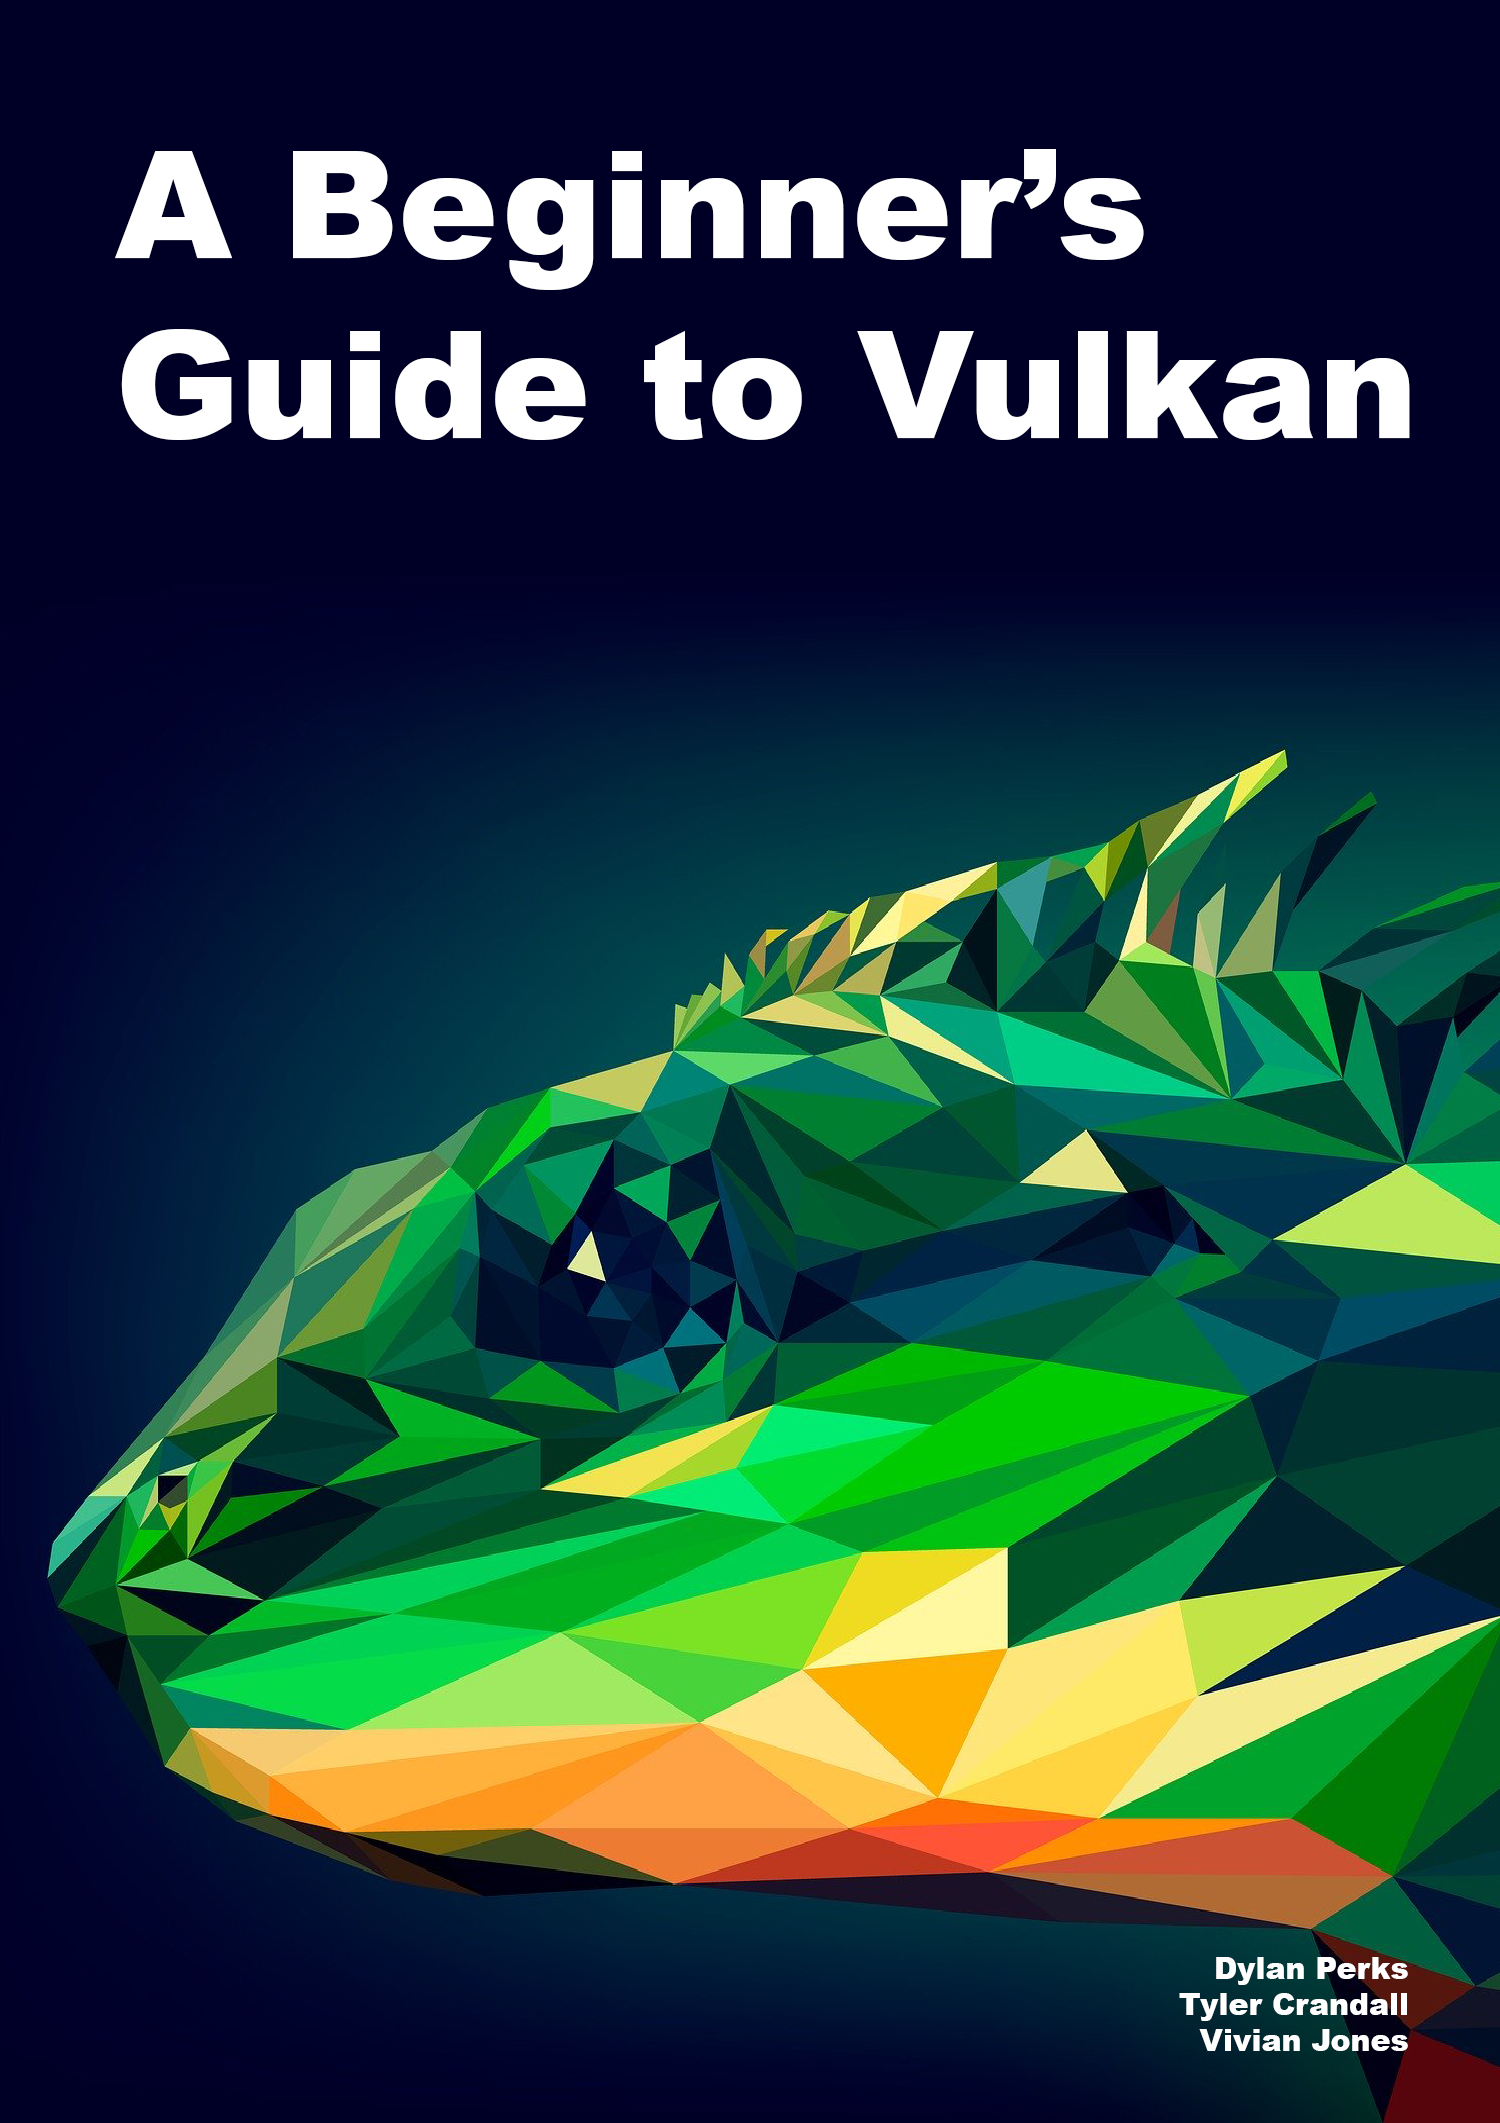
\includepdf[width=\paperwidth,height=\paperheight]{images/cover.png}
\newpage
\tableofcontents
%\chapter{Example}

This chapter is specifically made for demonstration on how to add various elements to the book and this chapter \textbf{SHOULD NOT} be included in the final copy of the book.

\begin{figure}[h]
    \centering
    \colorbox{backgroundcolor}{
        \parbox{0.9\textwidth}{
            \lstinputlisting[language=csh,style=csharp]
            {code/examples/Snippet1.cs}
        }
    }
    \caption{Example C\# Snippet}
    \label{fig:example_cs_snippet}
\end{figure}


Make sure to add figures.

\begin{figure}[h]
    \centering
    \colorbox{backgroundcolor}{
        \parbox{0.9\textwidth}{
            \lstinputlisting[language=GLSL]
            {code/examples/Snippet2.glsl}
        }
    }
    \caption{Example GLSL Snippet}
    \label{fig:example_glsl_snippet}
\end{figure}
\chapter{\textsf{Introduction}}
\chapter{\textsf{Mathematics Principles}}
\paragraph{}
For almost any non-trivial graphical program, geometry will need to be moved across the screen. The simplest way to do that would be to update the geometry's vertices to the new position, but constantly sending new data to the graphics card is very slow, and not feasible for a large-scale program.

\paragraph{}
In addition, Normalized Device Coordinates are too abstract for most graphical work. For example, drawing an image at the proper size is nearly impossible when all you have are NDC. Wouldn't it be easier to use a different coordinates system?

\par
The answer to both problems comes in the form of linear algebra. This chapter will be a \textbf{brief} introduction to the concept, and how it relates to graphics programming. If you find the topic interesting and want to know more, it is heavily recommended that you continue studying outside of this book. Several potentially-useful things (such as quaternions) are omitted here for brevity.

\par
With that said, let's begin!

\section{OpenGL Mathematics Library (GLM)}
\par
This tutorial is provided in C++, a language that does not include built-in linear algebra. Instead, we will use an external library: OpenGL Mathematics Library, or GLM for short. Despite the name, it will work for Vulkan just fine, as the mathematics required are the same. Download from here:

\par
\href{https://glm.g-truc.net/0.9.8/index.html}{https://glm.g-truc.net/0.9.8/index.html}

\par
At the time of writing, version 0.9.9.8 is the current stable release. If you encounter problems, be certain that you use the same version as we do.

\par
GLM is a header-only library, so no compiling or linking are necessary. Just download and copy the header folder into your includes folder.

\par
To ensure that it works, try running the following code:

\begin{figure}[h]
    \centering
    \colorbox{backgroundcolor}{
        \parbox{0.9\textwidth}{
            \lstinputlisting[language=csh,style=csharp]
            {code/chap2_MathematicsPrinciples/GLMTest.cpp}
        }
    }
    \caption{GLM test snippet}
    \label{fig:glm_snippet}
\end{figure}
\chapter{\textsf{Graphics Principles}}
\chapter{\textsf{Initial Setup}}
\chapter{\textsf{Shaders}}
\chapter{\textsf{Pipelines}}
\chapter{\textsf{Render Passes}}
\chapter{\textsf{Drawing}}
\chapter{\textsf{Project Guidance}}
\chapter{\textsf{Textures}}
\chapter{\textsf{Advanced Textures}}
\chapter{\textsf{Mapping}}
\chapter{\textsf{Instancing}}
\chapter{\textsf{Tessellation}}

\end{document}
